\chapwithtoc{Introduction}
	\ac{TPC} is a~type of gaseous detector that detects charged particle trajectories by measuring the~position and drift time of ions created in the~gas; details are provided in section~\ref{sec:tpc}. The~energy of such particles can be determined thanks to the~curvature of their trajectory in the~magnetic field.
	
	The~goal of this thesis is to develop an~algorithm for the~reconstruction of charged particle trajectories and energy in an~atypic \ac{TPC} (with orthogonal electric and magnetic fields, i.e., \ac{OFTPC}) used in the~X17 project at the~\ac{IEAPCTU}. Furthermore, we present the~results of testing this algorithm with different samples of simulated data. In the~future, we also plan to test this algorithm by measuring real particles with a~known energy distribution. In order to achieve this, we use the~Garfield++ toolkit~\cite{Garfield++} in combination with the~ROOT~framework~\cite{ROOT}. Some of our more demanding simulations are run on MetaCentrum.
	
	The~X17 project in \ac{IEAPCTU} aims to reproduce measurements of anomalous behavior in the~distribution of angular correlation of pairs produced by the~\ac{IPF} mechanism during the~decay of certain excited nuclei (\iso{Be}{8},~\iso{C}{12},~and~\iso{He}{4}) observed by the~ATOMKI group in Hungary. 
	
	\textcolor{red}{Add citations: MetaCentrum, X17 project, VdG, ATOMKI papers. Maybe also TPC, IPF, etc.}
	
	\section{ATOMKI Measurements}
	\textcolor{red}{Short summary of results of measurements in ATOMKI.}
	
	\section{X17 Project at IEAP CTU}
	\label{sec:IEAP}
		\textcolor{red}{Short summary of our goals, maybe mention the~grant.}
	
		\subsection{Our Detector}
		\textcolor{red}{Short description of our detector. Why we use an~atypic TPC. Gas mixture used in the~detector (70/30) and its effect.}
		
		\subsection{Magnetic Field Simulation}
		\textcolor{red}{Magnetic field simulations in Maxwell. Some figures. When working with the~magnetic field outside the~regular grid, we use trilinear interpolation.}
		
			\subsubsection{Trilinear Interpolation}
				Trilinear interpolation is a~generalization of linear interpolation in 3D. It can be used to interpolate a~function whose values are known on a~regular grid. We use this simple method for interpolating the~magnetic field, and it is also used in section~\ref{sec:grad} to interpolate the~Ionization Electron Map. In both cases, we use a~cubic grid.
				
				Let us consider a~cube (a~cell of our regular grid) with an~edge of length~$a$ containing the~point $C = (x,y,z)$ where we want to interpolate a~function $f\!\!:~\!\!\mathbb{R}^3\,\to\,X$ (\textcolor{red}{it should be better explained what $X$ is}). We know the~values of this function on the~vertices of this cube $C_{ijk} = (x_0+ia,y_0+ja,z_0+ka)$, where $i,j,k \in \{0,1\}$. We also define the~points $C_{ij} = (x,y_0+ia,z_0+ja)$ and $C_i=(x,y,z_0+ia)$. Then the~interpolated value $\widehat{f}(C)$ can be calculated as follows:
				\begin{equation}
					x_d = \frac{x-x_0}{a},~y_d = \frac{y-y_0}{a},~z_d = \frac{z-z_0}{a},
				\end{equation}
				\begin{alignat}{3}
					\widehat{f}(C_{ij}) &= (1-x_d)f(C_{0ij}) \,&+&\,x_d f(C_{1ij}),\\
					\widehat{f}(C_{i}) &= (1-y_d)\widehat{f}(C_{0i}) &+&\,y_d \widehat{f}(C_{1i}),\\
					\widehat{f}(C) &= (1-z_d)\widehat{f}(C_0) &+&\,z_d \widehat{f}(C_1).
				\end{alignat}
				
				\begin{figure}
					\centering
					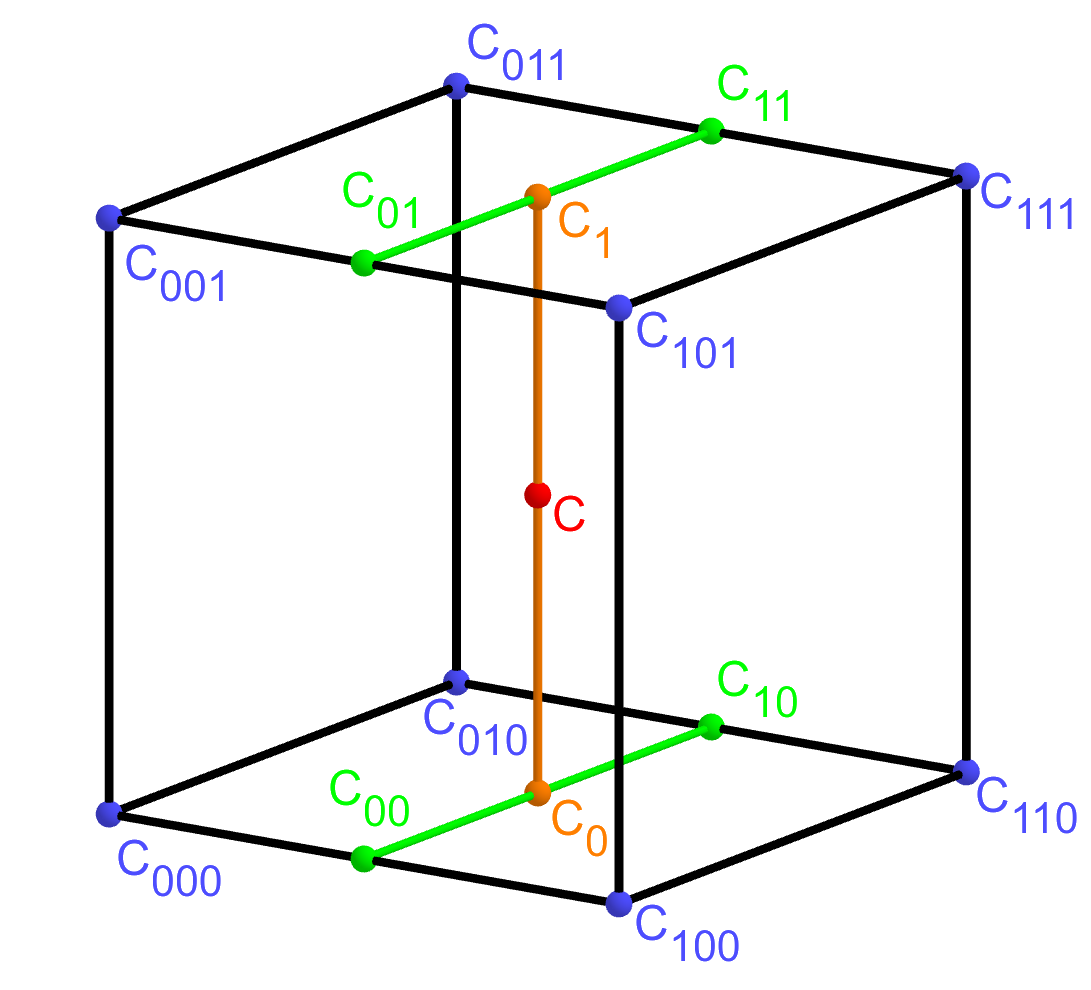
\includegraphics[width=0.5\textwidth]{trilinear.png}
					\label{fig:trilin}
					\caption{Visualization of trilinear interpolation. \textcolor{red}{Image drawn in GeoGebra and inspired by a~similar image on Wikipedia (looks a~bit worse) -- is credit necessary?}}
				\end{figure}
				
				\textcolor{red}{Maybe a~citation here, although I am not sure it is necessary since it could be considered common knowledge.}
		
		\subsection{Coordinate System}
		\label{sec:coor}
		\textcolor{red}{Description of the~coordinate system used in this thesis (+ figure). Introduce the~detector/readout space.}
	
	\begin{figure}
		\centering
		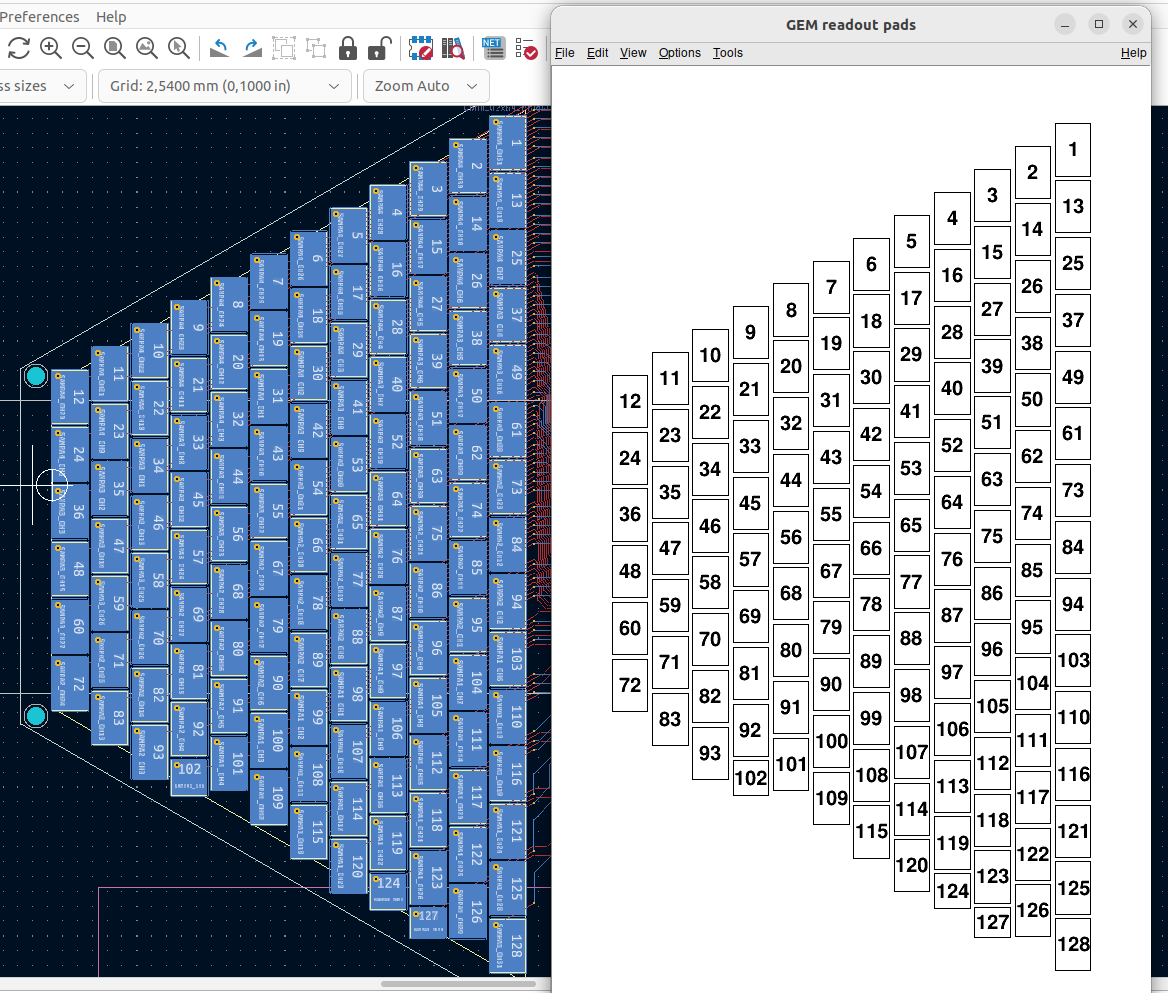
\includegraphics[width=0.8\textwidth]{padlayout.png}
		\caption{Pad layout of the~TPC. \textcolor{red}{Swap for better image.}}
		\label{fig:padlayout}
	\end{figure}